\section{Theoretical Foundations}
\label{sec:Theoretical_Foundations}
This section summarizes the theory and formulas necessary to understand the following experiments on the magnetic field in section \ref{sec:Evaluation}.

\subsection{Magnetic Flux Density}
\label{subsec:Magnetic_Flux_Density}
The decisive factor for the magnetic interactions is the magnetic flux density $\vect{B}$. In a vacuum or in the air, it is proportional to the magnetic field strength $\vect{H}$ \cite{magnetic_fields}.

The magnetic field strength $\vect{H}$ is used to calculate the magnetic flux density $\vect{B}$:
\begin{equation}
\vect{B}=\mu_0 \cdot \mu_r \cdot \vect{H} \qquad \text{with} \qquad
\begin{cases} 
	\mu_0=4\pi\cdot 10^{-7}\ \,^\text{Vs}\!/_\text{Am}\\
	\mu_r=1 \qquad \text{for vacuum or air} \\
\end{cases}
\label{eq:magnetic_flux_density}
\end{equation}
where:
\begin{conditions}
	\vect{B} & magnetic flux density \\
	\vect{H} & magnetic field strength \\
	\mu_0 & vacuum permeability \\
	\mu_r & relative permeability
\end{conditions}

\subsection{Calculating Magnetic Fields}
\label{subsec:Calculating_Magnetic_Fields}
The relationship between the electric current and the magnetic field generated by it can be formulated in two different ways. Either in an integral form with the Ampère's circuital law or in a differential form with the Biot-Savart law \cite{magnetic_fields}.
\addtocontents{toc}{\protect\setcounter{tocdepth}{2}}
\subsubsection{Ampère's circuital law}
\addtocontents{toc}{\protect\setcounter{tocdepth}{3}}
\label{subsubsec:Amperes_circuital_law}
Ampère's circuital law describes the total current $\Theta$ that passes through the area $A$, which is enclosed by the curve $\Gamma$ (graphically shown in figure \ref{fig:amperes_circuit_law}). The following formula is only suitable for the calculation of a symmetrical magnetic field, even though it is valid in any situation \cite{magnetic_fields}.
\begin{equation}
\Theta=\oint_\Gamma \,^{\vect{B}}\!/_{\mu} \cdot\vect{\text{d}l}=\oint_\Gamma \vect{H}\cdot\vect{\text{d}l}=\int \vect{j}\cdot \vect{\text{d}A}
\end{equation}
where:
\begin{conditions}
	\vect{B} & magnetic flux density \\
	\vect{H} & magnetic field strength \\
	\mu & permeability of a specific medium \\
	\vect{\text{d}l} & infinitesimal element of the curve $\Gamma$ \\
	\vect{j} & current density \\
	\vect{\text{d}A} & vector area of an infinitesimal element of the area A
\end{conditions}
\begin{figure}[H]
	\centering
	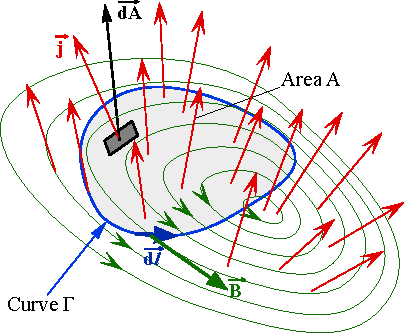
\includegraphics[scale=1]{amperes_circuit_law}
	\caption{Graphical representation of the Ampère's circuital law \cite{magnetic_fields} - partially modified}
	\label{fig:amperes_circuit_law}
\end{figure}
\addtocontents{toc}{\protect\setcounter{tocdepth}{2}}
\subsubsection{Biot-Savart law}
\addtocontents{toc}{\protect\setcounter{tocdepth}{3}}
\label{subsubsec:Biot-Savart_law}
The Biot-Savart law describes the contribution of a current path to the magnetic field at the point P. The resulting total magnetic field at the point P can be calculated by the integration over the whole conductor (graphically shown in figure \ref{fig:biot-savart_law}). This law can always be applied because it is based on the known geometry of the conductor \cite{magnetic_fields}.
\begin{equation}
\text{d}\vect{B}=\mu\cdot \text{d}\vect{H}=\frac{1}{4\pi|\vect{r}-\vect{r}_\text{L}|^2}\cdot\mu\cdot I\cdot\vect{\text{d}l}\times\frac{(\vect{r}-\vect{r}_\text{L})}{|\vect{r}-\vect{r}_\text{L}|}
\label{eq:biot-savart_law}
\end{equation}
where:
\begin{conditions}
	\vect{B} & magnetic flux density \\
	\vect{H} & magnetic field strength \\
	\mu & permeability of a specific medium \\
	I & current path \\
	\vect{\text{d}l} & infinitesimal element of the current path $I$
\end{conditions}
\begin{figure}[H]
	\centering
	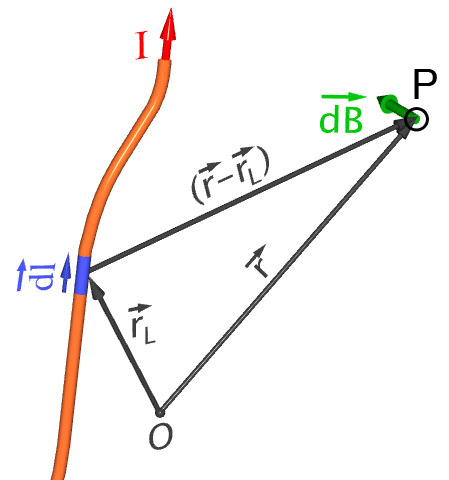
\includegraphics[scale=0.35]{biot-savart_law}
	\caption{Graphical representation of the Biot-Savart law \cite{magnetic_fields}}
	\label{fig:biot-savart_law}
\end{figure}
\newpage
\subsection{Measuring Magnetic Fields}
\label{subsec:Measuring_Magnetic_Fields}
The most common method to measure the magnetic flux density (see equation \ref{eq:magnetic_flux_density}) is to use a Hall effect sensor. A known current flows through a thin rectangular plate of a conductive material (usually a semiconductor). At the same time it is penetrated by the magnetic field $\vect{B}$. This results in an electrical field $\vect{F}_{\text{el.}}$ which is perpendicular to the current and the magnetic field. Furthermore, in equilibrium it compensates the Lorentz force $\vect{F}_L$. This means that the Lorentz force is equal to the electrical field ($\vect{F}_L=\vect{F}_{\text{el.}}$). The so-called Hall voltage can be measured at the narrow sides of the plate \cite{magnetic_fields}.
\begin{equation}
U_H=\frac{1}{N\cdot q\cdot d}\cdot I\cdot B\qquad \text{with}\qquad q=-e=-1.602\cdot 10^{-19}\ \text{C}
\end{equation}
where:
\begin{conditions}
	U_H & Hall voltage \\
	N & charge carrier density \\
	q & elementary charge \\
	d & thickness of the plate \\
	I & current \\
	B & magnetic field
\end{conditions}
Since the conductive material used in Hall sensors is usually a temperature-dependent semiconductor, alternating current (e.g. 1 kHz) is used to compensate thermoelectric voltages \cite{magnetic_fields}.
\begin{figure}[H]
	\centering
	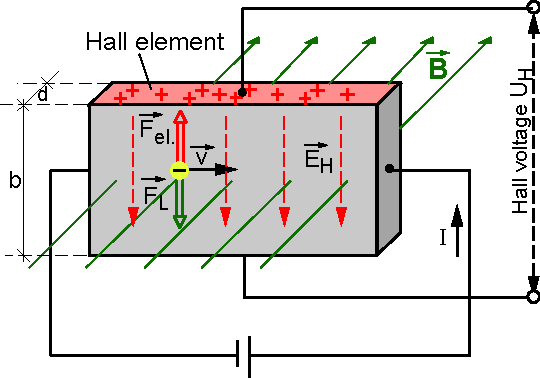
\includegraphics[scale=1]{hall_element}
	\caption{Construction of a Hall element \cite{magnetic_fields} - partially modified}
	\label{fig:hall_element}
\end{figure}

\subsection{Cylindrical Coil}
\label{subsec:Cylindrical_Coil}
For the derivation of the magnetic field of a cylindrical coil, it is assumed that the coil is of length $l$, with a diameter of $2R$ and $N$ turns (one or two layer wound). For the construction see figure \ref{fig:cylindrical_coil}. The following derivation is based on the Biot-Savart law (see equation \ref{eq:biot-savart_law}) \cite{magnetic_fields}.

First, the discrete winding current is replaced by an equivalent surface current $j_{2-d}$:
\[
N\cdot I=l\cdot j_{2-d}
\]
This results in a current segment with the length $\text{dz}_\text{L}$ which represents a cylindrical coil with the radius $R$ and the current:
\[
\text{d}I=j_{2-d}\cdot \text{dz}_\text{L}
\]
Its contribution to the magnetic field at the point P is:
\[
\text{d}B_z=\frac{\mu_0\cdot R^2}{2}\cdot\frac{\text{d}I}{\left[(z-z_\text{L})^2+R^2\right]^{\,^{3}\!/_{2}}}=\frac{\mu_0\cdot N\cdot I \cdot R^2}{2l}\cdot\frac{\text{dz}_L}{\left[(z-z_\text{L})^2+R^2\right]^{\,^{3}\!/_{2}}}
\]
To obtain the magnetic field $B$ at the position $z$, one has to integrated over the entire length of the coil (from $\,^{-l}\!/_{2}$ to $\,^{+l}\!/_{2}$):
\[
B_z(z)=\frac{\mu_0\cdot N\cdot I \cdot R^2}{2l}\cdot\int_{\,^{-l}\!/_{2}}^{\,^{+l}\!/_{2}}\frac{1}{\left[(z-z_\text{L})^2+R^2\right]^{\,^{3}\!/_{2}}}\cdot\text{dz}_L
\]
This results in the following equation for the magnetic field $B_z$:
\begin{equation}
B_z(z)=\frac{\mu_0 N I}{l}\cdot\frac{1}{2} \left[\frac{\,^{l}\!/_{2}+z}{\sqrt{(\,^{l}\!/_{2}+z)^2+R^2}}+\frac{\,^{l}\!/_{2}-z}{\sqrt{(\,^{l}\!/_{2}-z)^2+R^2}}\right]
\label{eq:cylindrical_coil_bz}
\end{equation}
To obtain the magnetic field in the center of the coil $B_z(z=0)$, the following equation is used:
\begin{equation}
B_0=B_z(0)=\frac{\mu_0 N I}{l}\cdot \frac{1}{\sqrt{1+(\,^{2R}\!/_{l})^2}}
\label{eq:cylindrical_coil_b0}
\end{equation}
where:
\begin{conditions}
	B_z & magnetic field at the position z \\
	B_0 & magnetic field in the center \\
	\mu_0 & vacuum permeability \\
	N & number of turns \\
	I & current \\
	l & length \\
	z & position \\
	R & radius
\end{conditions}
\begin{figure}[H]
	\centering
	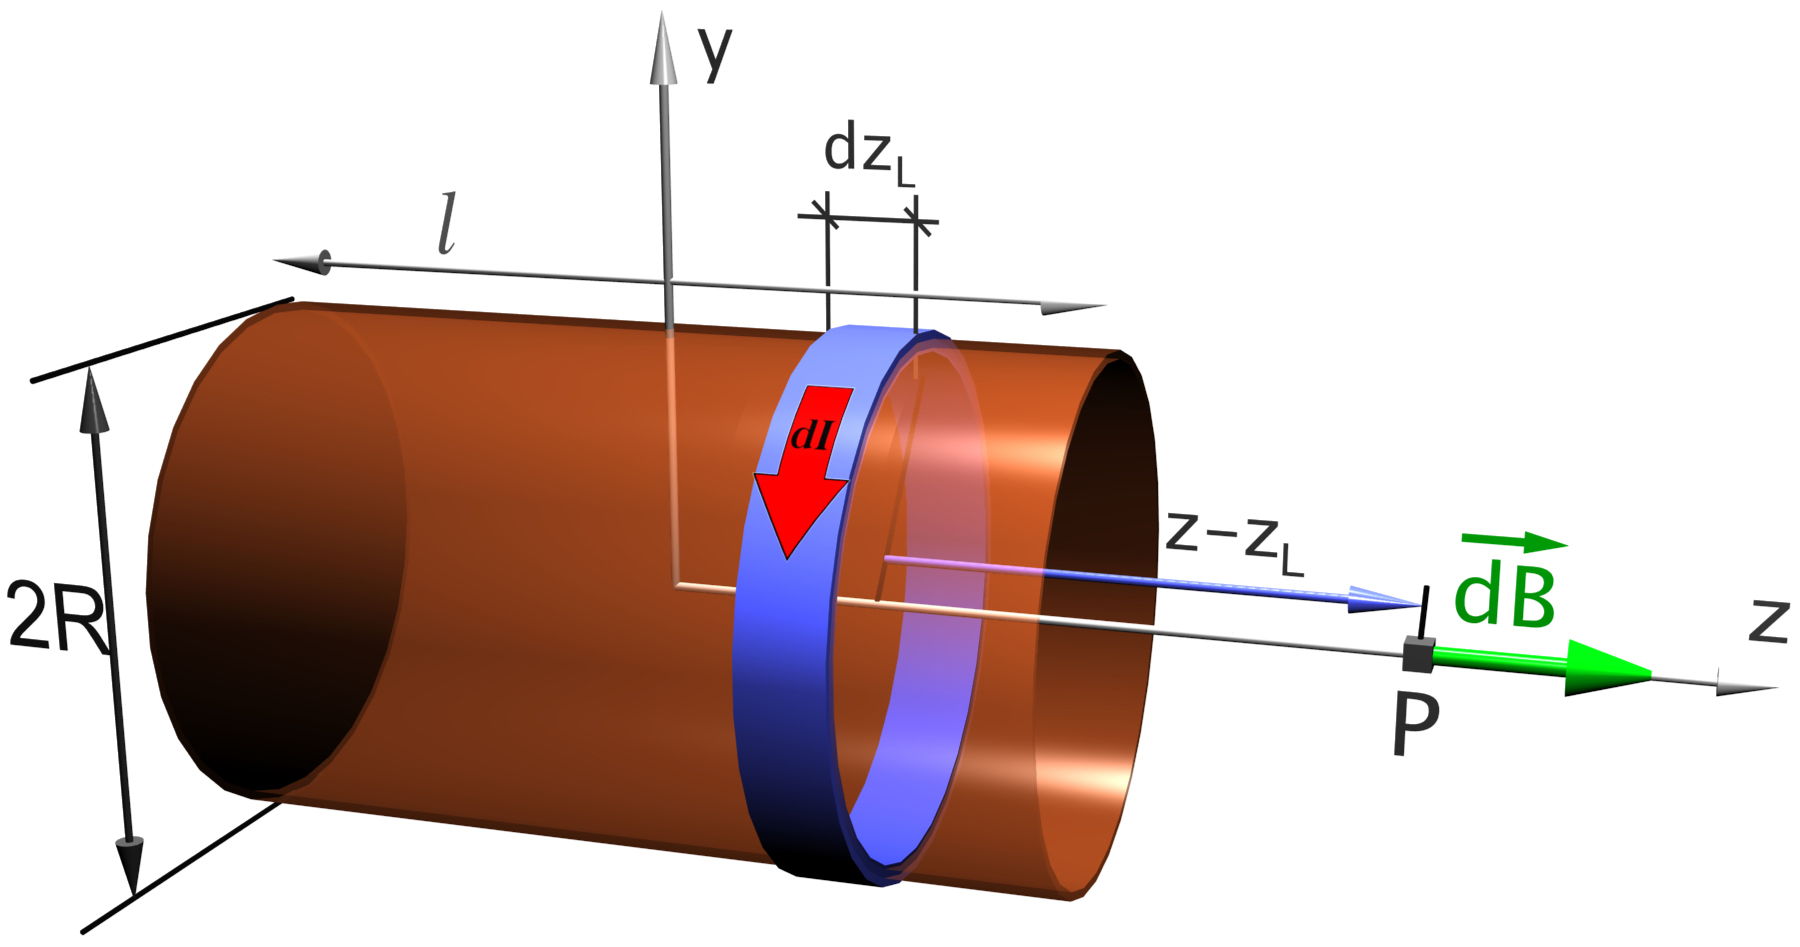
\includegraphics[scale=0.25]{cylindrical_coil}
	\caption{Construction of a Cylindrical Coil \cite{magnetic_fields}}
	\label{fig:cylindrical_coil}
\end{figure}
